\documentclass[a4paper,14pt]{extarticle}
\usepackage{geometry} % Bigger font size for article

% make it more readable non-serif
\usepackage{lmodern}
\usepackage[T1]{fontenc} % i.a. makes title font non-serif
\renewcommand{\familydefault}{\sfdefault}
\usepackage{titlesec}

%monospace font command for codes
\usepackage{alltt}
\def\code#1{
	\begin{alltt}
	\texttt{#1}
	\end{alltt}
}

%remove newline after subsubsection sections
\usepackage{titlesec}
\titleformat{\subsubsection}[runin]{\normalfont\normalsize\bfseries}{\thesubsubsection}{1em}{}

% reduce numbering
\setcounter{secnumdepth}{2}

% hungarian language
\PassOptionsToPackage{defaults=hu-min,classmod=unchanged}{magyar.ldf}
\usepackage{t1enc}
\usepackage[magyar]{babel}
\selectlanguage{magyar}
\usepackage[utf8]{inputenc}

% compacitem
\usepackage{paralist}


% images 
\usepackage{graphicx}
\graphicspath{ {./images/} }

% set smaller margins
\addtolength{\oddsidemargin}{-1.2cm}
\addtolength{\evensidemargin}{-1.2cm}
\addtolength{\textwidth}{2.4cm}
\addtolength{\topmargin}{-1.5cm}
\addtolength{\textheight}{3cm}

% remove red color for hyperref in TOC (maybe only in Adobe reader)
\usepackage[unicode]{hyperref}
\hypersetup{
	colorlinks,
	citecolor=black,
	filecolor=black,
	linkcolor=black,
	urlcolor=black
}

\begin{document}
	
	\begin{titlepage}
	\begin{center}
		{\LARGE\textbf{Nagyvállalati szoftverfejlesztés Java alapon vizsga kérdések}}
	\end{center}
	\vfill
	\begin{center}
		{\large Utoljára módosítva: \today}
		\vspace{0.5cm}
		
		{Készítette: Ráncsik Áron}
	\end{center}
\end{titlepage}
	
	\tableofcontents
	\newpage
	\section{SOLID elvek nagyvállalati gyakorlatban}
		\subsection{Mit jelentenek a következő fogalmak?}
			\subsubsection{Encapsulation}
			Egységbezárás, az adatok és a rajtuk végzett műveleteket, OOP esetén osztályokba zárjuk.
			
			\subsubsection{Abstraction}
			Elhagyunk a kontextus számára nem fontos dolgokat, és csak az adott feladat számára lényeges információ kivonattal dolgozunk. 
			\par Amit nyerünk: 
			\begin{compactitem}
				\item Komplex dolgok egyszerű kezelése
				\item Modellezés
				\item Duplikáció elkerülése
			\end{compactitem}
			
			\subsubsection{Inheritance}
			\label{inh}
			Öröklődés. Legerősebb kapcsolat két osztály között.
			\par Előnyei: 
			\begin{compactitem}
				\item Kód újrafelhasználás.
				\item Modellezésben: általánosabb dolgokat ki lehet szervezni ősosztályba
				\item Ősosztály több, független kiterjesztésére alkalmas.
			\end{compactitem}
			
			\subsubsection{Polimporphism}
			Többalakúság. Különböző típusok egy interfaceként való kezelése.
			\par Megvalósítása: 
			\begin{compactitem}
				\item Függvény túlterhelés.
				\item Generikus programozás.
				\item (OOP) függvény felülírás leszármaztatottban.
			\end{compactitem}
		
		\subsection{Milyen relációkat ismersz? Mi az a kompozíció?}
			\subsubsection{Inheritance} 
			Öröklődés. lásd: \ref{inh}
			\subsubsection{Interface Implementation}
			Interface implementáció. Hasonló az öröklődéshez, de gyengébb a kapcsolat. Interface nem tartalmaz implementációt.
			\subsubsection{Composition}
			Mező, attribútum egy osztályban. Egy osztály egy másik osztályra hivatkozik.
			Létrehozás és megszüntetés is a létrehozó osztály feladata.
			\subsubsection{Aggregation}	
			Mező, attribútum egy osztályban. Egy osztály egy másik osztályra hivatkozik.
			Az osztály csak használni tudja ha kap egy példányt. Nem tartozik a felelősségébe a példány létrehozása.
			\subsubsection{Associacion}
			Mező, attribútum egy osztályban. Egy osztály egy másik osztályra hivatkozik.
			Az osztály \textbf{opcionálisan} csak használni tudja a másik objektumot, de ha null lenne a hivatkozás akkor is működőképes marad nélküle.
			\subsubsection{Dependecy}
			Egy osztály módosítása esetlegesen kihathat egy másik osztály módosítására. Egy osztály dependál, ráépít, támaszkodik egy másik osztályra.
			
		\subsection{Ismertesd a SOLID elveket}
			\subsubsection{{\Large S}ingle Responsibility} 
			Egy osztálynak egy felelőssége legyen. És ez a felelősség lehetőleg ebben az egy osztályban legyen egysége zárva.
			\newline
			Egy osztálynak egy oka legyen a változásra.
			\newline
			Előny:
			\begin{compactitem}
				\item Könnyebben lehet kezelni az osztályokat változó környezetben. Robusztus.
				\item Kisebb lesz a kohézió egy osztályon belül. A felelősségek szétválaszthatóak lesznek. 
			\end{compactitem}
		
			\subsubsection{{\Large  O}pen/Closed} 
			Osztályok, entitások lehetőleg legyenek nyitottak a bővítésre és zártak a módosításokra.
			\newline
			Zártság célja, hogy az osztályok módosítását elkerüljük. Arra törekszünk ne keljen az osztályt módosítani.
			\newline
			Nyíltság: Arra törekszünk, hogy bővítés esetén minimális módosításra legyen szükség.
			\newline
			Megoldás: Használjunk absztrakciót.
				
			\subsubsection{{\Large  L}iskov substitution}
			Liskov féle helyettesítési szabály.
			Leszármaztatott osztály csak olyan módosításokat csinálhat ami nem változtatja az ősosztály felelősségét és működését. A leszármazott osztály példány helyettesíthető legyen az ősosztály példánnyal.
			Ha ősosztályként tekintek egy leszármaztatott osztályra nem szabad, hogy különbséget lássak, továbbra is működjön úgy ahogy egy ősosztály példány is működne.
			Feltételek:
			\begin{compactitem}
				\item \textbf{ Metódus szignatúrák egyezése} (Java nyelvben alap).
				\item \textbf{ Preconditions.} Paraméterként átadott adatokkal kapcsolatos elvárások megtartása, csak erősíteni lehet. Pl. ha ősosztály működik null paraméterrel a akkor a leszármaztatott is működjön.
				\item \textbf{Postconditions.} A visszaadott eredmény nem szegheti meg az ősosztály által nyújtott garanciákat.
				\item \textbf{Invariánsok.} Ilyen értéket nem módosíthatjuk meg. Pl. Ha az ősosztály egy értéket nem módosított egy bizonyos metódus hívásra akkor lehetőleg a leszármazott se módosítsa azt.
				\item \textbf{History constarint.} A leszármazott nem módosíthatja olyan formában a belső állapotot ami megzavarja az ősosztály működését.
			\end{compactitem}
		
			\subsubsection{{\Large  I}nterface segregation}
			Klienseket nem kéne olyan függőségekre kényszeríteni amire nincs szükségük.
			Pl. Interface rengeteg metódussal, de ebből csak néhányat szeretnénk használni. Szerep alapú interfacek legyenek.

			C++ esetén: header interface helyett szerep interface. Lustaságból lehetne a header fájlt interfacnek használni, de ne tegyük ezt.
			\par Előny:
			\begin{compactitem}
				\item Kevésbé lesz egybefüggő a kód.
				\item A változásokra kevésbé lesz érzékeny az implementáló kód.
			\end{compactitem}
		
			\subsubsection{{\Large  D}ependency inversion}
			Magas-szintű moduloknak nem lenne szabad függeniük az alacsony-szintű moduloktól.
			Mind kettőnek absztrakcióktól kellene függeniük.
			
			Régi szokás (volt) magas-szintű modulokat alacsony-szintű modulokra építeni.
			Ehelyett sokkal jobb, ha egy absztrakciós réteget hozunk létre a magas- és az alacsony-szintű réteg közé, tehát interfaceektől függjenek. Egy magas-szintű modul alacsony-szintű függőségeit pedig konstruktoron keresztül oldjuk fel.

			Ebben az esetben viszont az a kérdés merül fel, hogy a függőségeket melyik rétegben példányosítsunk, erre megoldás az Inversion Of Control (röviden IoC) container. bővebben: \ref{di}
			
		\subsection{Mit jelentenek a következők?}
			\subsubsection{Demeter szabály}
			Egy objektum ''A`` kérhet szolgáltatásokat (metódus hívással) ''B`` objektumtól, de ''A`` objektumnak nem kéne ''B`` objektumot csak kihasználva ''B`` től elkérnie egy másik ''C`` objektumot, hogy aztán az ''A` a ''B``-n keresztül, `''C``-től kérjen szolgáltatásokat. Ebben az esetbem ''A`` ismeri a ''B`` belső szerkezetét és ez nem jó.
			\par Előny:
			\begin{compactitem}
				\item Rejtett függőség elkerülése.
				\item Kezelhetőbbé adaptálhatóbbá válik az osztály.
			\end{compactitem}
		
			\subsubsection{Tell, don't ask principle}
			Ha egy objektum több hívás végez egy másik objektumon egymás után, egy feladat elvégzésére akkor azt a másik objektumot "kérdezgeti", ehelyett, a másik objektum egy metódushíváson keresztül kiszolgálhatnánk a hívó kódot.
			
			Mondjuk meg egy objektumnak, hogy mit csináljon, ne pedig az adatait kérdezgessük le, hogy utána megcsináljuk.
			
			\subsubsection{KISS} Keep it simple stupid. Amennyire lehet egyszerűsítsünk, ne bonyolítsuk feleslegesen a kódot.
			
			\subsubsection{YAGNI} You ain't gonna need it.
			Ne fejlessz olyan dolgok amire nem lesz szükség.
			
			\subsubsection{Immutable és Value objektum}
			Immutable:(C\# esetén megfeleltethető a primitív, egszerű típus) nem megváltoztatható objektum. ''final`` mező. Szálbiztos, egyszerűen érthető, de módosításhoz le kell másolni
			\newline Value: (C\# esetén referencia típus)
			Referencia értéket tárolunk.
			Pl. Egyenlőséget belső állapot alapján vizsgáljuk pl. String equals
			
	\section{Gyakori tervezési minták nagyvállalati gyakorlatban}
	Tervezési minta egy bevett gyakorlat, sok év programozói tapasztalat alapján kialakult jó szokások, bevett megoldások, minták. Adott problémát, mintát felismerve egy "best practise", hogyan kell ezt megoldani.
		\subsection{Létrehozási (creational) tervezési minták}
			Célok:
			\begin{compactitem}
			\item Egységbe zárni azt az ismeretet ami a létrehozáshoz kell, pl. az objektum belső felépítését pl. más objektumokra hivatkozását szeretnénk egyetlen helyen kezelni. Később csak ezen az egy helyen kell majd módosítani.
			\item El akarjuk rejteni egy osztály konkrét implementációját.
			\end{compactitem}
			Pl. Sok osztályban inkább csak egyetlen létrehozó osztálytól akarunk függeni, mint sok sok létrehozást duplikáltan létrehozni a sok osztályban.
			\par Objektum vagy osztály alapú kategóriái vannak.
			
			\subsubsection{Builder pattern}
			Az objektumot felépítését a reprezentációjától szeretnénk elkülöníteni.
			A builderben ''beállító `` metódusok és egy ''build `` metódus van. A builder Kompozícióval hozza létre a kívánt osztályt.
			Egy osztálynak lehet több buildere ezeknek kell egy közös builder ősük.
			
			\subsubsection{Factory method}
			Készítsünk egy létrehozó osztály interfacet és az ebből leszármaztatott osztályok döntsék el hogy milyen konkrét példányt készítenek. Virtuális konstruktor.
			Van egy osztály legyen ''F`` ami (egy metódusa) létrehoz egy objektumot, de ez a metódus visszatérésként absztrakt osztályt interfacet ad vissza, de ''F`` osztály leszármazottai ezt felül definiálják és más más konkrét implementációval térnek vissza.
			
			\subsubsection{Static factory method}
			Az osztálynak csak privát konstruktora van, de van egy statikus pl. "newInstance" metódusa amivel létre tud hozni magából egy példányt. pl. Calendar osztály. pl. Ha új szálat akarunk indítani egy konstruktorban ami nem jó, mert akkor még nincsenek a mezők inicializálva, ehelyett, ezzel a mintával ezt megoldhatjuk.
			
			\subsubsection{Simgleton pattern}
			Azt szeretnénk, hogy egy osztályból egyetlen példány készüljön, de ehhez szeretnénk globális hozzáférést biztosítani.
			Statikus létrehozó metódus mindig ugyanazzal a példánnyal tér vissza.
			Többszálú környezetben figyelni kell a konkurens hozzáférés helyes megvalósítására.
			Általában előbb-utóbb több példányra lesz majd szükség, ezért érdemes ezt olyan keretrendszerre bízni ahol könnyen leváltható ennek a mintánk a használata.
			
			\subsubsection{Abstarct Factory}
			Factoryt gyártó factory, termékcsaládok legyártására.
			
			\subsubsection{Prototype pattern}
			Felkonfigurált objektumot másolással bővítjük (tipikusan JS)
			\newline Depp copy = rekurzívan minden kompozit osztályt adattagjaival együtt lemásolunk. \newline Shallow copy = a hivatkozott osztálynak csak a hivatkozását másoljuk így a másolat és az eredeti osztály is ugyanarra az osztályra fog hivatkozni. 
			
		\subsection{Szerkezeti (structural) tervezési minták}
		Hogyan érdemes strukturálni az objektumainkat.
		Kisebb objektumokat szeretnénk egy komplexebb feladat elvégzésére össze strukturálni.
		\newline Cél:
		\begin{compactitem}
			\item Flexibilis kód.
			\item Változásra való felkészülés.
		\end{compactitem}
		Ezek a minták  jellemzően delegációra és kompozícióra építkeznek.
			\subsubsection{Adapter pattern}
			Az adapter kényszerhelyzetet orvosol. Pl egy interface és egy implementációt nem illik össze akkor közéjük rakunk egy adaptert. Meglévő megoldást adaptálunk saját használatra.
			Az adapter általában compozit kapcsolattal hivatkozik az adoptálandó objektumra. 
			
			\subsubsection{Bridge pattern}
			Válasszuk szét az absztrakciót az implementációtól.
			Az ötlet hogy öröklés helyett kompozícióval hivatkozzunk az implementációra. Futásidőben lehet cserélni az implementációt.
			Absztrakció csak továbbít. Az öröklés hátrányaitól megszabadulunk. Ha egy környezetben függetlenül módosul az absztrakció pl. a hogy mit várnak el a kliensek, és a az implementáció, hogy ezt hogyan valósítjuk meg akkor érdemes használni.
			pl. sql.DriverManager
			
			\subsubsection{Decorator pattern}
			Plusz felelősséggel szeretnék dinamikusan bővíteni az osztályt. pl. streamek egymásba ágyazása.
			
			\subsubsection{Facade pattern}
			Egységes, egyszerű hozzáférést biztosít egy bonyolult alrendszerhez. Egy interfce, több interface számára egy alrendszerben. Magasabb szintű hozzáféréssel egyszerübbé teszi az alrendszer használatát. pl. JPA, rétegek közötti kommunikáció könnyítésére használják.
			
			\subsubsection{Proxy pattern}
			Helyettest biztosítunk egy objektumra. Pl. Hozzáférés kontrollálására használjuk. Közös interface. Általában csak továbbít plusz funkciót nem végez.
			pl. Lazy loading.
			
			\subsubsection{Composite pattern} Rész egész viszony leképezésére van pl. xml DOM. rekurzív használata.
			
			\subsubsection{Flyweight pattern} Optimalizációs céllal jött létre. Ha egy objektumra gyakran szükség van, és sokat nyerhetünk azzal ha több kliens is ugyanazt az objektumot használja.
			
		\subsection{Viselkedési (behavioural) tervezési minták}
			Objektumok közötti kommunikációt és az összetett felelősség felosztását szeretnénk megtenni. Laza kapcsolatot szeretnénk, ezért főleg kompozíciót fogunk használni.
			
			\subsubsection{Command pattern}
			Egy kérést ne metódus hívás jelképezzen, hanem zárjuk a kérést egy objektumba.
			Szétválaszthatjuk a hívás és a végrehajtást. Fontossági sorrendet alakíthatunk ki.
			Kérés sorokat hozhatunk létre (batch) és visszavonási műveletet valósíthatunk meg.
			
			\subsubsection{Iterator pattern}
			Kollekció elemeihez szeretnénk úgy hozzáférést biztosítani, hogy ne kelljen felfedni a kollekció belső szerkezetét. External: Iterátor készül egy kollekcióhoz. Az iterátor belelát az kollekcióba, általában belső osztály. Pl hashmap esetén nem lehet elkerülni a használatát.
			
			\subsubsection{Mediator pattern}
			Sok-sok objektum kommunikál egymással valamilyen gráffal ez leírható. Ahelyett hogy, az összes objektum ismerje az összes másik objektumot, jól jöhet egy mediátor, közvetítő aki a objektumok közti kommunikációért felelős. A mediátort mindenki ismeri, a mediátor pedig ismeri az összes kommunikálni kívánó osztályt. És az objektumok ha egymással akarnak kommunikálni akkor a mediátorhoz fordulnak.
			
			\subsubsection{Observer pattern}
			Több-több kapcsolat objektumok közötti kommunikációban. Ha egy objektum állapota megváltozik akkor ez az objektum minden erre a változásra feliratozott objektumot értesít a változásról.
			
			\subsubsection{Strategy pattern}
			Definiálunk egy algoritmus családot, különböző algoritmusokat egységbe zárjuk és így egymással felcserélhetővé tesszük az algoritmusokat. pl. Layout manager.
			Közös interface az összes támogatott algoritmusoknak. Egy kontextusból tudja az algoritmus a számára szükséges adatokat megszerezni. Nagyon hasonló osztályok esetén, amiknek a  viselkedése csak kicsit különbözik, akkor érdemes használni, kódismétlés elkerülésre.
			
			\subsubsection{Template method}						
			Vázat adunk egy algoritmusra és a leszármazottak, és a leszármazottak csak egy-két lépést felül definiálnak, de a vázat megtartják. Öröklést használunk. \newline Pl. servlet. \newline 
			Final matódus legyen amit nem lehet felüldefiniálni, de amit kell azt absztrakt metódusba rakjuk.
			
	\section{Verziókezelési stratégiák, git flow}
		\subsection{Mik a verziókezelés előnyei?}
			Változtatások nyilvántartása: ki, mikor, mit változtatott.
			Korábbi állapot megtekintése, visszatérés rá.
			\subsection{Mit jelent az elosztott verziókezelés?}
			A lényeg, hogy nem egy központi helyen vezetjük adatok változtatását. Változtatások lokális kezelése mások megzavarása nélkül. Egy gépen is megtalálható a teljes változás követés összes változata.
			\subsection{Milyen Git parancsokat ismersz?}
			\begin{compactitem}
				\item config
				\item init
				\item clone
				\item status
				\item add
				\item commit
				\item push/pull
				\item branch
				\item checkout
				\item merge
				\item rebase
				\item reset
			\end{compactitem}

		\subsection{gitk, .gitignore mire való?}
			\subsubsection{gitk}
			Grafikus program githez ami a commitokat és brancheket tudja megjeleníteni.
			\subsubsection{.gitignore}
			Ebben a fájlban felsorolhatjuk a verziókezelésből ignorálni kívánt fájlok nevét. Csak arra a mappába és annak almappáira vonatkozik ahol létrehozzuk.
		\subsection{Mit jelent a távoli repository?}
		Az a kitüntetett repo amihez hozzá tud férni több munkatárs is arra használják, hogy lokális módosításaikat szinkronizálják. Általában szolgáltató adja pl. Github, Gitlab, BinBucket
			\subsubsection{Hogyan lehet kommunikálni vele?}
			git remote add távoli repository hozzáadása lokális repohoz, cloneozáskor megtörténik automatikusan. majd pl. a lokális master branch trackeli a remote master branchet. 
			Pull és push segítségével lehet műveleteket végezni, kommunikálni.
		\subsection{Mi az a Pull/Merge request?}
		Mind kettő jelentése: Egy fork branch vissza mergelése az eredeti repoba.
		
		Nem a git , hanem a git menedzselő alkalmazás része ez a funkció. GitHub: pull request, GitLab: merge request. Csak a nevük különbözik.
		\subsection{Mi a különbség a merge és a rebase között?}
			\subsubsection{Merge} Két ág összefűzése, a két ág külön külön megmarad és egy merge committal kerül egybe.
			\subsubsection{Rebase}
			Egy ág összes commitját átmozgatjuk egy új ágba.
			\subsubsection{Mikor melyiket érdemes használni?}
			Erről vallásháborúk vannak.
			A rebase akkor jó, ha lineáris commit historyt szeretnénk. Általában ha egy kisebb 1-2 fős csapat dolgozik, egy feature branchen akkor ott rebase-t használhatnak, \textbf{de közös megosztott branchen nagyon nem ajánlott a használata.} Merge együtt tartja az összetartozó komitokat, de az linearitás sérül, én merge párti vagyok.
		\subsection{Ismerted a tréning anyagban szereplő branching modellt}
			master, develop, feature, release, hotfix
			\newline
			\begin{center}
				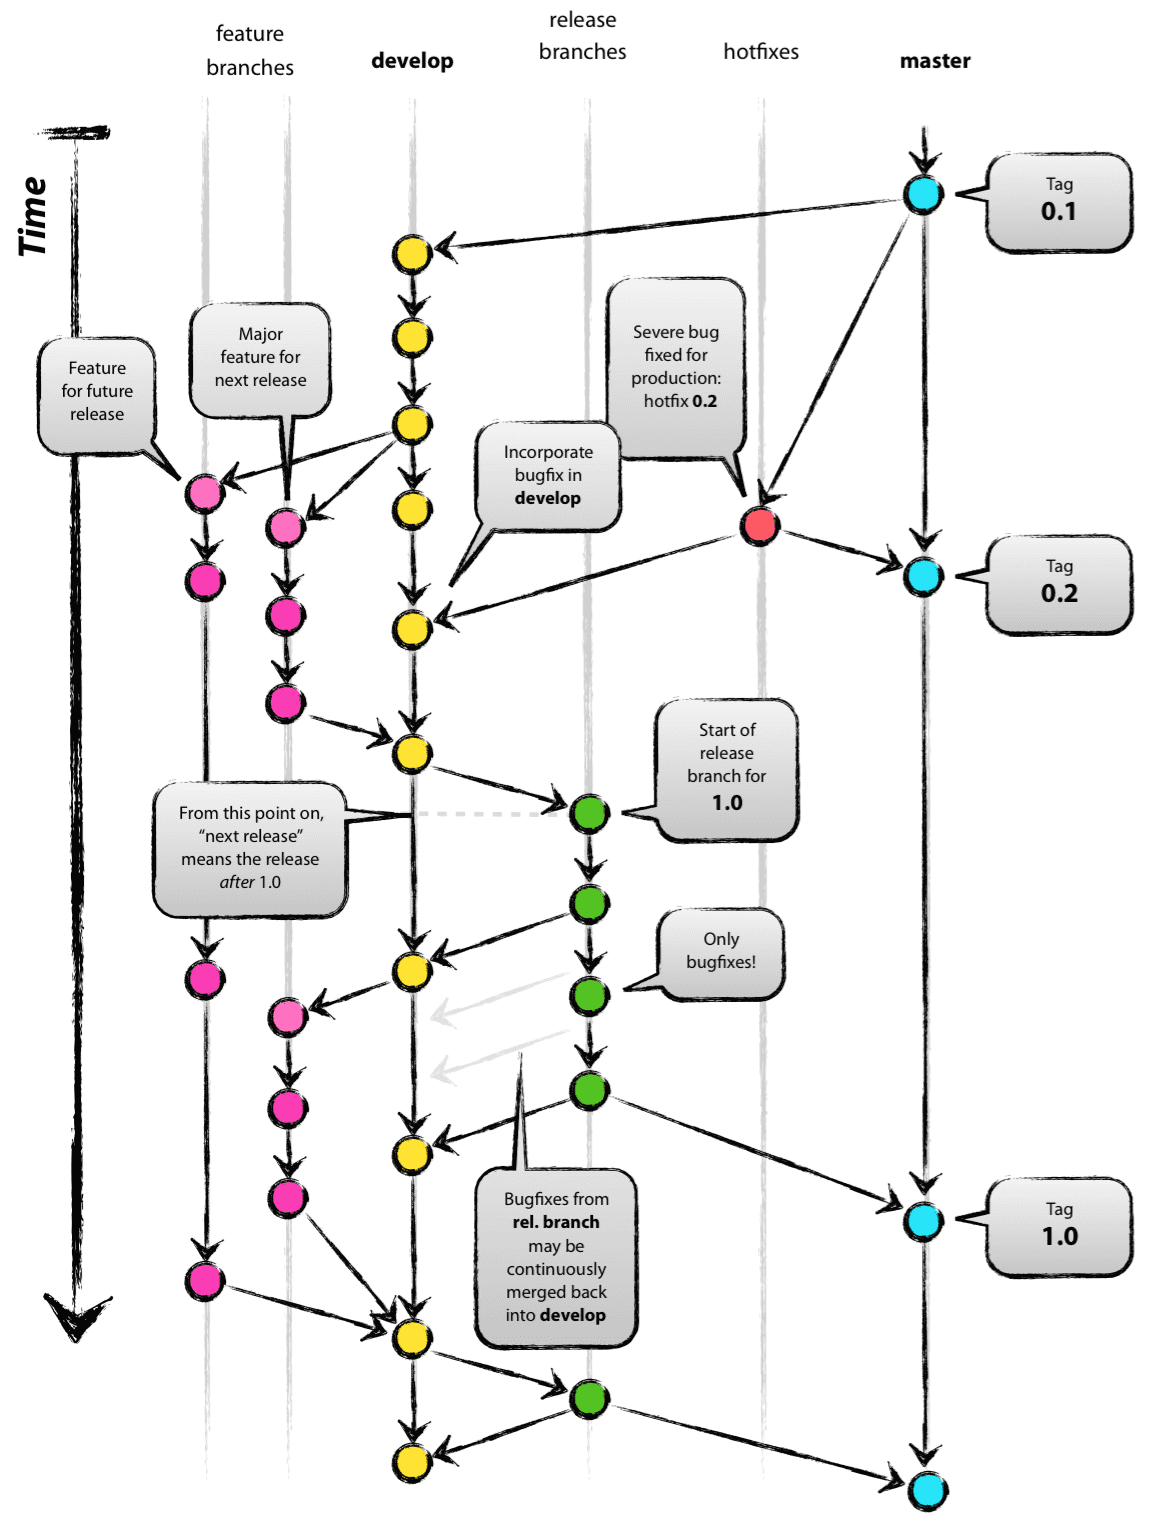
\includegraphics[width=10cm]{gitbranching}
			\end{center}
		\subsection{Milyen Git workflow-kat ismersz? }
		\begin{compactitem}
			\item Egyszerű egy közös központi repoba pusholás.
			\item Integration-manager workflow 
			\newline
			\begin{center}
				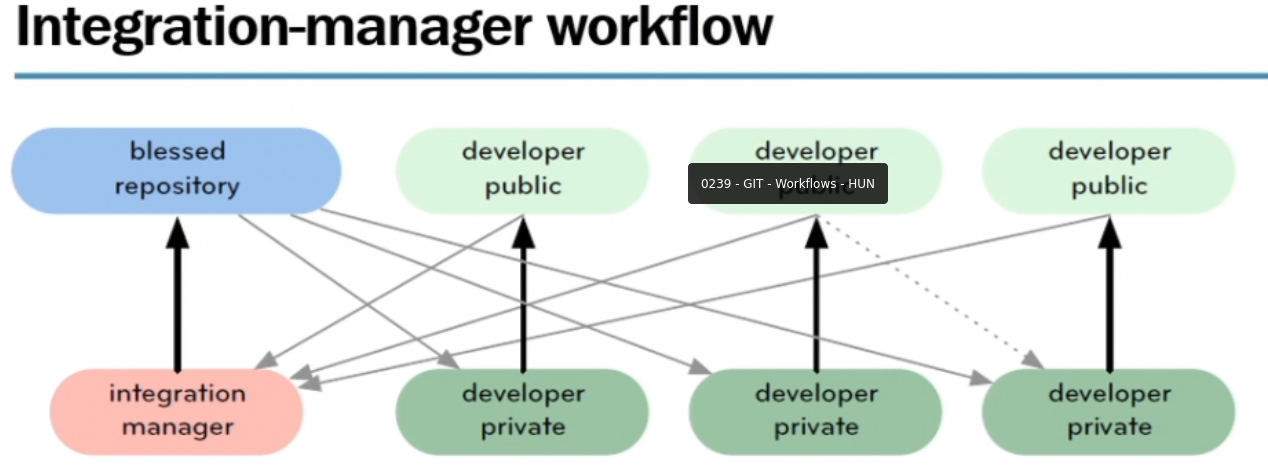
\includegraphics[width=10cm]{imwf}
			\end{center}
			Integration manager-en keresztül lehet a fő repot módosítani.
			\item Diktátor workflow
			\newline
			\begin{center}
				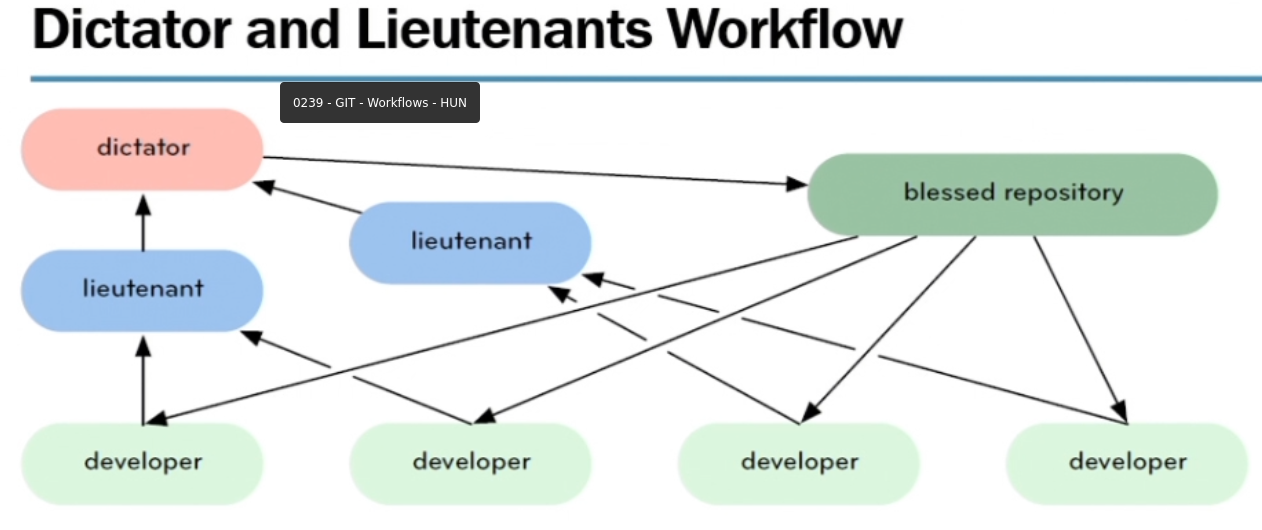
\includegraphics[width=10cm]{dictator}
			\end{center}
			
		\end{compactitem}
			
	\section{XML és JSON}
	Dokumentum leíró nyelvek.
		\subsection{XML fogalma}
		eXtensible Markaup Language
		\subsection{Mit jelentenek a következő fogalmak?}
			\subsubsection{XML TAG}
			Egy elem a fa szerkezetben.
			pl. \code{<button>b</button>} 
			\subsubsection{Attribútum}
			Egy elemnek lehet tulajdonsága.
			De a gyerekelem jobban bővíthető, módosítható.
			pl. \code{<button attr="asd">b</button>}
			\subsubsection{Jól formázott XML (well formed}
				\begin{compactitem}
					\item Nyitótag lezárása kötelező.
					\item Elemek lezárásának sorrendje a nyitás sorrendjével (fordítottan) egyezzen, ne legyen overlap.
					\item Egy gyökér elem legyen.
					\item Attribútumok értékek legyenek kódolva. Védett karakterek.
					\item Egy attribútum kétszer ne legyen megadva.
					\item Komment és tag nem keresztezheti egymást.
				\end{compactitem}
		
			\subsubsection{XSD}
				XML Séma Definíció 
				\newline Egy leírás tervrajz arra hogy hogyan kell kinéznie, milyen tageket attribútumokat tartalmazhat egy dokumentum ami a adott sémát megvalósítja.
				A séma készítéshez is van egy séma.
			\subsubsection{Valid XML}
				Egy adott sémának való megfelelés.
		\subsection{Milyen XML feldolgozási módokat ismersz?}
		JaxP java API for XML processing
			\subsubsection{DOM parsing}
				Egész XML dokumentumot a memóriában kezeli, nagyon kényelmes, de sok memóriát használ.
				Véletlenszerű hozzáférés az összes elemhez, módosítani lehet a fát. 
			\subsubsection{Push parsing SaX / JAXP}
			Egyszer végig fut a dokumentumon és eseménykezelők definiálásával lehet kezelni. Read-only, lineáris bejárás, nincs random hozzáférés. Eseményeket kapunk a parsertől, hogy milyen elem jött, majd eldönthetjük, hogy azzal mit akarunk csinálni.
			\subsubsection{Pull parsing StaX}
			Hasonló események mint Push esetén. Plusz
			cursorral iterátorral lehet mászkálni.
			Read-only, lineáris bejárás, nincs random hozzáférés.
			Ezek eddig túl alacsony-szintűek.
		\subsection{Mi a JaxB?}
			Java API for XML binding.
			Kényelmes, ezt szeretjük használni.
			Marshal: Java object to XML
			Unmarshal: XML to Java object.
			Kell xml kell séma és fel kell annotálnia az osztályunkat.
			\newline xjc sémából osztály generál annotálva.
	\section{Build eszközök, Maven}
		Apache Maven is a software project management and comprehension tool. Based on the concept of a project object model (POM), Maven can manage a project's build, reporting and documentation from a central piece of information. 
		\subsection{Mit jelent a build automatizálás?}
			A buildelést nem manuálisan végezzük, hanem van erre egy program, szkript vagy eszköz amit elindítva megcsinálja ezt automatikusan.
			\subsubsection{Miért hasznos?}
			A manuális buildből származó emberi hibákat letudjuk csökkenteni.
			Bonyolult bild folyamatok kód generálást is használnak pl DAO, ezekhez konfigurációkat interfaceket használnak, ezeket becsomagolják, ez rengetek munka lenne kézzel. Ennek a segítségével megvalósítható a continuous integration (CI). Ha új kódot írunk egyből ellenőrizhetjük CI segítségével, hogy minden okés-e, és nem kell megvárni a release-t.
		\subsection{Mire való Maven esetén a pom.xml fájl?}
			Egy projekt teljes leírását tartalmazza.
			Projekt Objektum Mapping.
			\subsubsection{Mit írunk bele?}
			\begin{compactitem}
				\item Verzió
				\item Group id
				\item Artifact id
				\item Java könyvtár függőségek.
				\item Modul függőségek.
				\item Esetleges ős modulból való leszármazás.
				\item Repository kezelés
			\end{compactitem} 
			\subsubsection{Mit jelent a convention over configuration?}
				Egy maven config alapértelmezetten a már mindenki által ismert, kialakult szokás alapján van beállítva és csak az ettől való eltérést kell megadni deklaratív formában.
			\subsubsection{Mi az a fázis, plugin, goal, lifecycle?}
				A Maven életciklusa a következőképp írható le: \newline
				Vannak nagy fázisok. A fontosabbak: validáció -> compile -> test -> package -> integration-test -> verify -> install -> deploy
				Pl. A compile fázisban a compiler plug-int használjuk. A compiler plug-innak vannak góljai. pl. compile goal vagy testCompile goal. 
				\begin{center}
					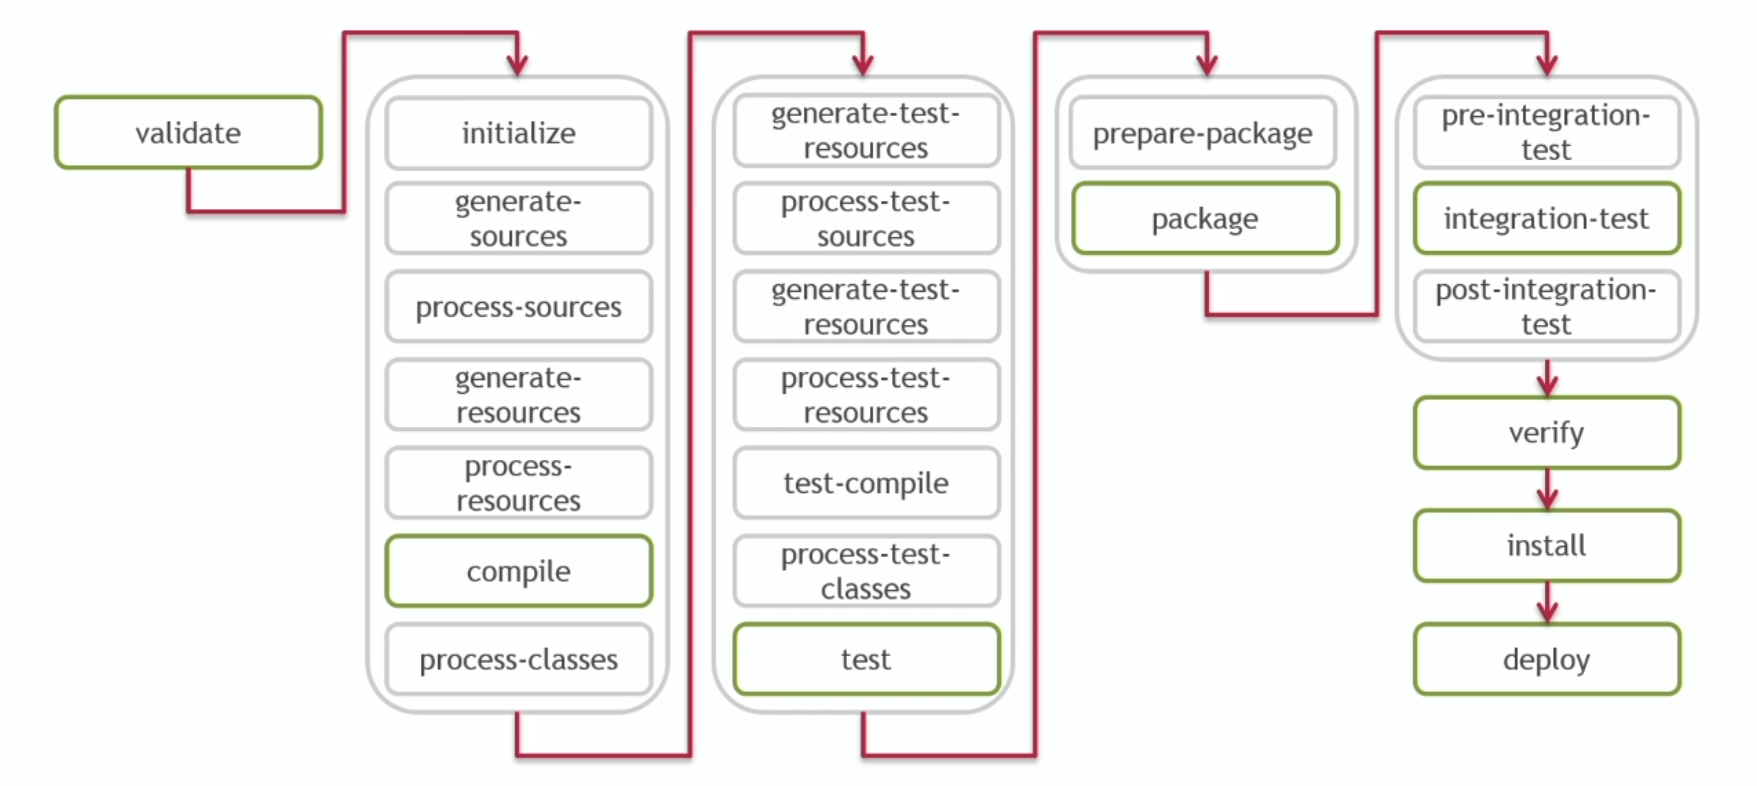
\includegraphics[width=13cm]{mavenlifecycle}
				\end{center}
	
	\section{Java keretrendszerek, a Spring alapjai}
		\subsection{Mit jelent a dependecy injection (DI)?}
		\label{di}
			"Függőség beinjektálás." Keretrendszer végzi. A DI a IoC egy konkrét megvalósítása.
			\subsubsection{Milyen előnyei vannak?}
				\begin{compactitem}
					\item A függőség létrehozásának felelősségétől megkíméljük a DI-t használó osztályt.
					\item A létrehozás egy helyen van leírva, így könnyen módosítható később, mert nincs kód duplikáció.
					\item Singleton minta könnyen használható.
				\end{compactitem}
			\subsubsection{Spring esetén milyen fajtáit ismered?}
			\begin{compactitem}
				\item Konstruktor paramétereket,
				\item Settert,
				\item vagy mezőt is lehet injektálni, de nem javasolt.
			\end{compactitem}

		\subsection{Mi a Spring bean?}
			Olyan java objektum aminek a létezéséről a  Spring tud, és Spring IoC konténer kezeli (pl. létrehozza, stb.).  
		\subsection{Mi a Spring bean definíció (config)?}
		Egy leírás egy konkrét bean objektumra, ami alapján a Spring létre tudja hozni ha szükséges konkrét beaneket objektumokat.
		Függőségeket is itt lehet megadni.
		\subsection{Mi a Spring bean-ek életciklusa?}
		\begin{compactitem}
			\item Inicializáció
			\item Használat
			\item Megszüntetés
		\end{compactitem}
		\begin{center}
			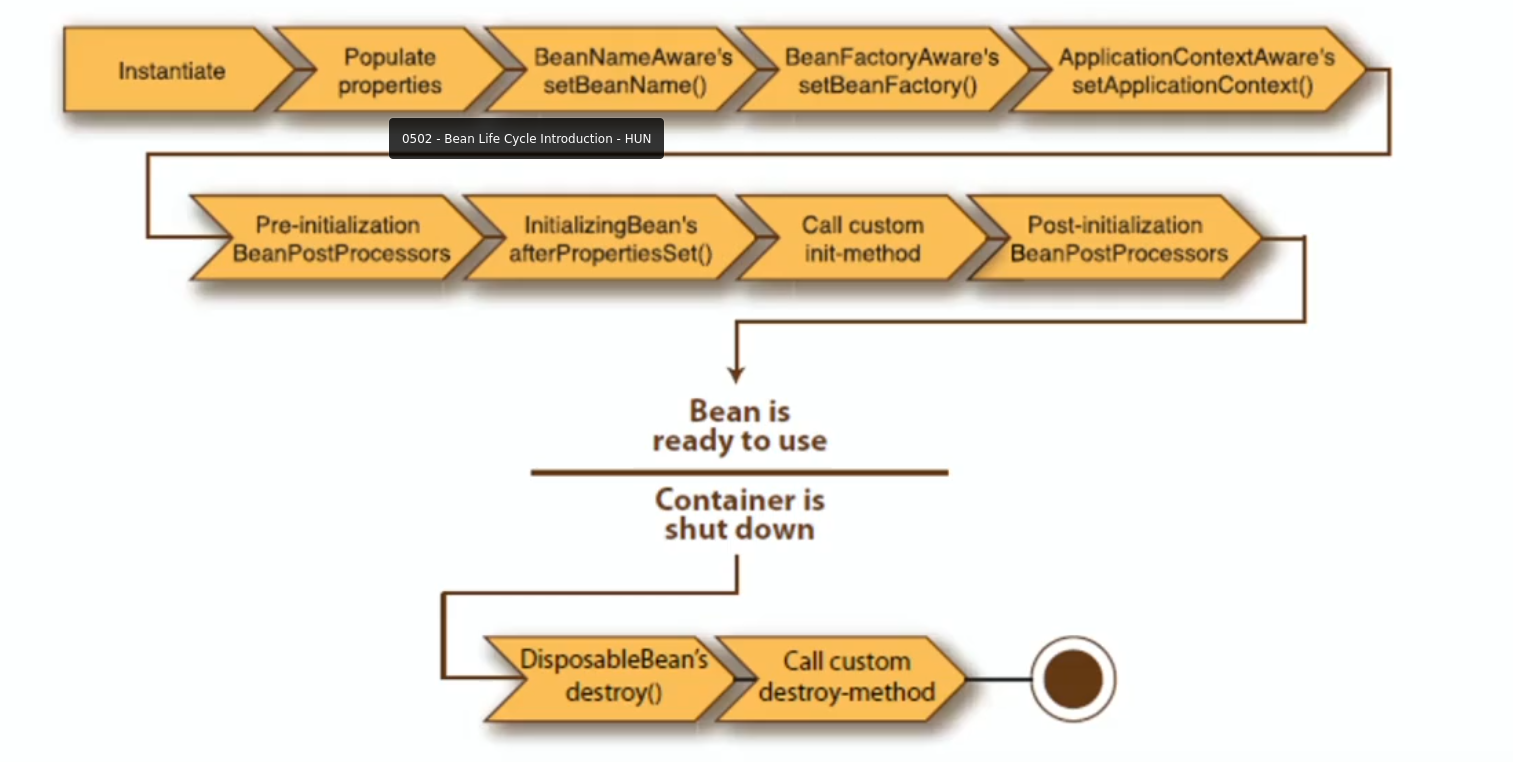
\includegraphics[width=13cm]{beanlifecycle}
		\end{center}
		Pl.
		\newline Singleton (alapértelmezett): A beanből egy példány jön létre.
		\newline Prototype: Mindig amikor szükséges újat hoz létre a bean definició alapján.
	
	\section{Spring keretrendszer részletei, spring framework}
		\subsection{Mit jelent Spring esetén autowire?}
		Egy annotáció, aminek a segítségével tudunk függőséget beinjektálni oda ahova a kitesszük. Bean (config) definícióban lehet használni.
		\subsection{Mi az a BeanFactoryPostProcessor, Factory Bean?}
		PostProcesszor: lefut a bean életciklus lépései között, ennek a segítségével hozzá lehet adni kiegészítő kódokat a bean életciklushoz. Ezzel lehet Beant proxyzni, wrappelni kiegészíteni, dekorálni. 
		Factory Bean: Spring megvalósítása  a factory method viselkedésnek.
		\subsection{Milyen konfigurációs módokat ismersz?}
			\subsubsection{XML}
			Egy séma alapján lehet XMLben Beaneket definiálni.
			\subsubsection{Java}
			Java osztály @Configuration nnotációval ellátva @Bean annotált metódusokkal lehet Beaneket létrehozni.
			\subsubsection{Annotáció}
			DI is megvalósítható a komponenseken, belül annotációval így nem kell elkülönített config fájl ennek kezelésére.
			\subsubsection{Melyiknek mik az előnyei, hátrányai?}
			Annotációval nem lehet mindent megcsinálni kicsit szétszórtabbá teszi a konfigurációt, de így is sokkal kényelmesebb mint az XML. Java konfig is sokkal kényelmesebb mint az XML, és mindent meg lehet vele csinálni. XML alapú konfig, régi módszer,mindent meg lehet vele csinálni ,fordítás nélkül lehet módosítani ennyi az egyetlen előnye.
			
	\section{Adatelérési eszközök (JDBC)}
		\subsection{Mire való a JDBC API?}
			Különböző adatbázisokhoz való csatlakozásra, adatküldésre és fogadásra használjuk. DriverManager kiválasztja a megfelelő drivert a választott adatbázishoz (url alapján), és létrejön a kapcsolat.
			Csinálunk egy statementet amin tudunk queryt futtatni.
			A query futtatásának eredménye ResultSet lesz.
			\subsubsection{Miért nem kényelmes a használata?}
			Hibakezelés macerás: vendor specifikus hibakódokat ad csak vissza.
			CheckException, Resource bezárás kell.
			\subsubsection{Milyen kiegészítést ad a Spring a használatához?}
			\begin{compactitem}
				\item DAO support: különböző megvalósítások egységes kezelése.
				\item JdbcTemplate: DAO support JDBC fölé csak a lényeges queryt kell megírni a többit elintézi.
				\item Egységes exception hierarchia, csak runtime exception.
			\end{compactitem}
	
	\section{Fejlett adatelérési eszközök (jpa, spring data)}
		\subsection{Mire való a JPA?}
		JPA egy szabvány amit lehet implementálni. Pl. konkrét implementációja a hibernate.
		Java persistent API
		\newline
		Cél: objektumok és relációik perzisztenssé tétele az adatbázisba. 
		\subsection{Mit jelent a configuration by exception?}
		Egy csomó alapértelmezett beállítás van pl. tábla neve az osztály neve lesz stb. és csak ezektől való eltérést kell konfigurálni.
		\subsection{Milyen főbb annotációkat ismersz?}
			\subsubsection{@Entity} Annotált osztály entitás lesz.
			\subsubsection{@Id} Annotált mező lesz a primary key.
			\subsubsection{@Column} Annotált mező  oszlop neve állítható.
			\subsubsection{@Basic LAZY} Betöltés csak hivatkozás esetén.
			\subsubsection{@Enumeration} Enumot el tud tárolni, string vagy szám alapján.
			\subsubsection{@Temporal} Date esetén lehet időt vagy dátumot vagy timestampet tárolni.
		\subsection{Hogyan valósítható meg reláció a JPA segítségével?}
		\subsubsection{Single-valued associations}
		Én hivatkozok \textbf{egy} másik entitásra, ha csak én akkor @OneToOne , ha rajtam kívül más is @OneToMany annotáció kell.
		\subsubsection{Collection-values associations}
		Ha nálam egy kollekció és azokra csak én hivatkozok akkor @ManyToOne ha azokra más is hivatkozhat akkor @ManyToMany annotáció kell.
		\subsection{Milyen módokon támogatja az öröklődést a JPA}
			\subsubsection{Singe table} Egy nagy táblában az összes leszármazott plusz egy mező, hogy milyen típusú az rekord.
			\subsubsection{Join table} Összerakja külön táblákkal kibővíti az ősosztályt.
			\subsubsection{Table per class}
			Ősosztály mezői plusz az új mezők külön táblákban.
			
		\subsection{Mi az a Spring Data}
			Még magasabb szintű adatbázis támogatás. pl. Spring Data JPA.
			Interface alapú programozás modell.
			Metódus név lapján generál implementációt.
			Deklaratív lekérdezés lefuttatás.
			\subsubsection{Milyen szolgáltatásokat ad a JPA-hoz képest?}
			Repo build JPA alapján. Type-safe JPA lekérdezés.
			Transparent. Lekérdezés validáció bootstrap (spring épülés) közben.
	\section{Webfejlesztés – web alapok, servlet, jsp}
		\subsection{Mi a különbség egy webszerver és egy alkamazásszerver között?}
		Webszerver kifejezetten HTTP tartalom kiszolgálására van. Alkalmazás szerver képes HTTP tartalmat kiszolgálni, de nincs megkötve csak erre pl. FTPt is kiszolgálhat.
		\subsection{Hogyan épül fel egy HTTP request és egy response?}
		\begin{compactitem}
			\item URL
			\item metódus típus: GET, POST, PUT, DELETE, stb
			\item Header: pl. content/type, agent, session stb.
			\item Paraméterek: get, post formában key-value párok.
		\end{compactitem}

		\subsection{Mire való a servlet és a JSP?}
		\subsubsection{Servlet} Egy API. Ennek egy implementációja pl. a tomcat, glassfish. Az az API ami a hálózattal való kapcsolattartást definiálja.
		\newline Servlet egy web komponens amit a szerverre deployolunk hogy dinamikus weboldalk készítsünk.
		\subsubsection{JSP}
		JavaServer Pages.
		Egy HTML szerű leírása az oldalnak, dinamikus adatok által vezérelt alkalmazást lehet a segítségével készíteni. Servletre épül és servletre fordul.
		\subsection{Mire való a web.xml?}
			A szerver bejövő request kezelését lehet benne konfigurálni.
		\subsection{Mire jók a Scope-ok?(application, session, request)}
			\subsubsection{request} Beant készít egy request erejéig.
			\subsubsection{application} Beant készít a webszerver kontextus életciklusába.
			\subsubsection{Session} Beant készít ami a session létezéséig fog létezni.
		\subsection{Mire jó egy cookie?}
		Kliens oldalon el tudunk benne tárolni kulcs-értékpárok formájában adatokat. Amik böngésző újraindítás esetén is megmaradnak. pl session id. tárolása.
	\section{Webfejlesztés - spring boot és spring mvc alapok}
		\subsection{MVC fogalma}
		Model, View, Controller.
		Egy minta.
		Három aspektus, modul, réteg.
		View ismeri a modelt.
		A Controller is ismeri a modellt.
		A Conroller ismeri a viewt is.
		\begin{center}
			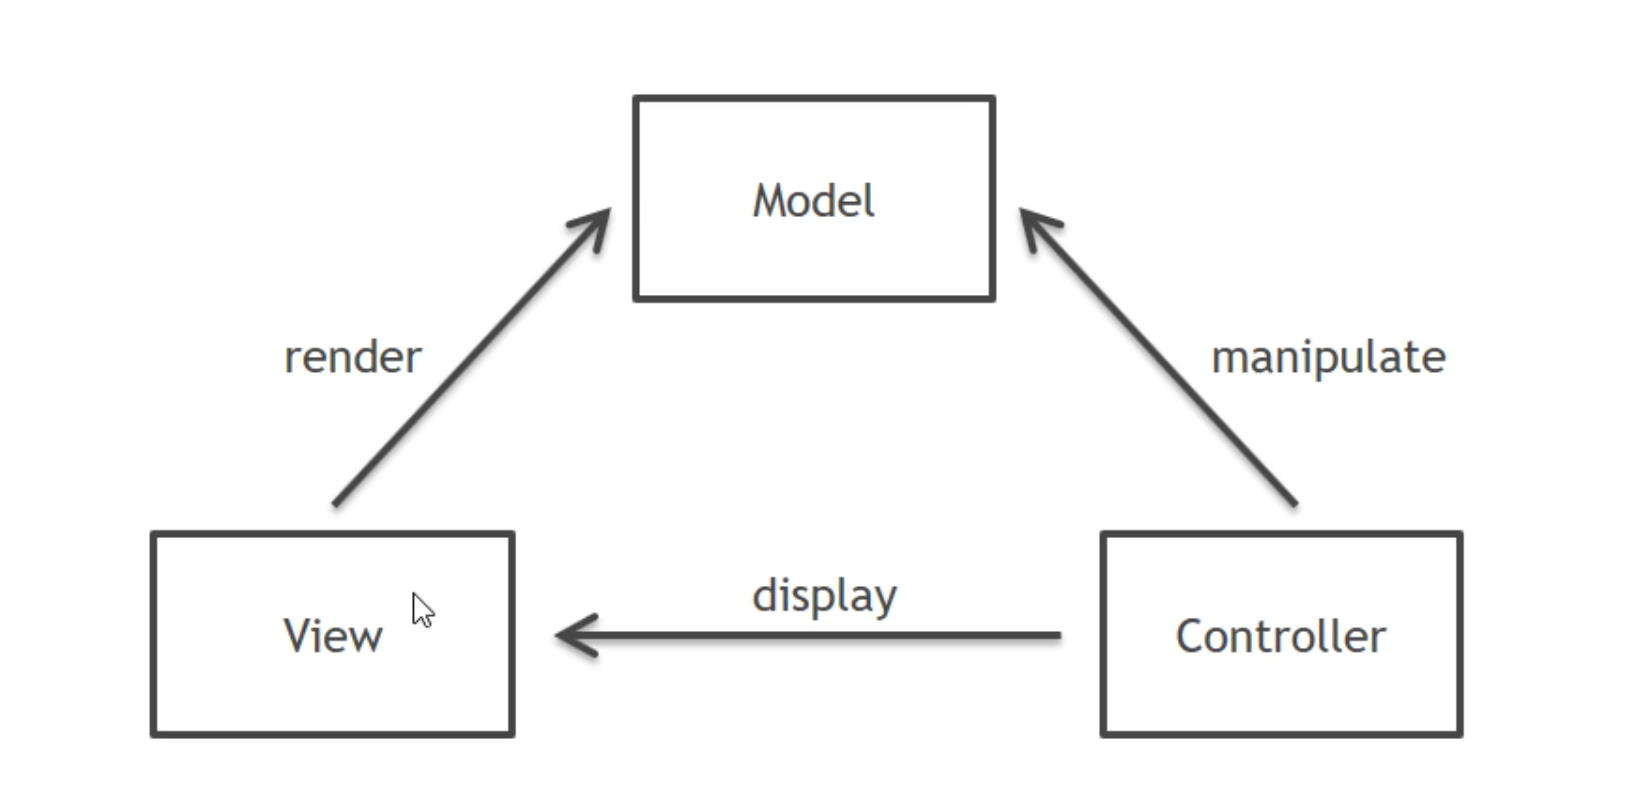
\includegraphics[width=13cm]{mvc}
		\end{center}
		\subsection{Spring MVC project létrehozása Spring Boot segítségével}
		A spring boot egy eszköz ami arra lett kitalálva, hogy spring mvc framworköt használó alkalmazást lehessen készíteni gyorsan. Azonnali konfigurációkat tartalmaz, Spring alapú alkalmazás elindításához. stb. 
		\subsection{@Controller feladata}
		Megkapja a requestet, készít egy modelt és egy megjelenítésnek tovább adja.
		\subsection{Tipikus MVC  hívási lánc}
		JSP -> controller -> service -> repository -> domain 
		\subsection{Security konfigurálása MVC segítségével (login form, WebSecurityConfigurerAdapter)}
		Egy Spring modul aminek a beiktatásával az oldalt elérését belépéshez köthetjük. Egy kijelölt Login és Register oldalak elvégzik az autentikációt. A Spring security pedig alapvető fontos biztonsági beállításokat, nem engedi az oldal elérést autentikáció nélkül.
		\subsection{Mi az a MockMVC?}
		MCV kérés-válaszokat lehet vele tesztelni.  A tesztelés céljára konfigolja fel az MVC-t (nem kell teljesen).
	\section{Webfejlesztés –java alapú webes technológiák, spring mvc}
		\subsection{Többrétegű alkalmazás tipikus felépítése}
			\begin{compactitem}
				\item{ 
					Web 
					\begin{compactitem}
						\item JSP
						\item Controller
						\item Model
					\end{compactitem}	
				}
				\item Service
				\item Repository
				\item Domain
			\end{compactitem}
		\subsection{@Controller request mapping}
			Egy kontroller tipikusan egy request kezelésére van.
			A request mapping meghatározza, hogy milyen requesteket kezeljen a kontroller.
		\subsection{request processing lifecycle}
		\begin{center}
			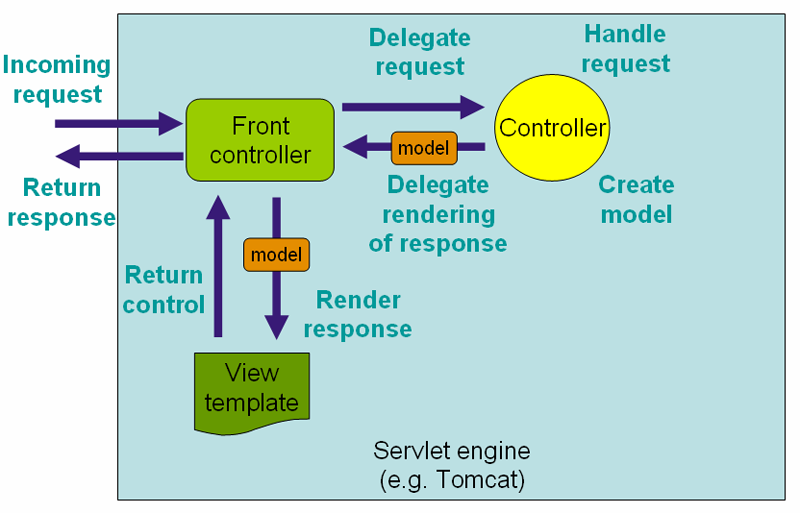
\includegraphics[width=13cm]{req}
		\end{center}
		\subsection{Data binding}
		Adatkötés. request paramétereket név alapján domain objektumra tudja kötni. 
		\subsection{Spring taglib}
		Egy JSPben használható könyvtár. pl. Két irányú adatkötést tud készíteni egy Spring form és data objektum között. 
		\subsection{Form-ok létrehozása}
		Spring form tag használata után elérhető. 
		\code{%
			<\%\@ taglib prefix="form" uri="..." \%>
			\newline
			<form:form ... >
		}
		\subsection{CSRF védelem}
		Egy példa:\newline
		A böngészőben az egyik tabon be vagyunk jelentkezve a Bankba, és egy másik tabon mondjuk facebookon valaki készit egy gombot ami a háttérben a következőt linket nyitja meg: 
		\verb|bank.hu/utalas?ide=123&ennyit=9999| akkor mivel be vagyunk lépve csak egy másik tabon akár le is futhatna kérés, ez ellen akarunk védelmet, hogy a mi alkalmazásunkat, még ha be is van lépve, ilyen linkekkel ne lehessen utasítgatni más oldalak által.  
		\subsection{REST fogalma}
		Representational state transfer. Architektúra stílus. Egy köteg megszorítás egy webszolgáltatás elkészítésére, ha ezeket a megszorításokat betartjuk akkor az alkalmazásunkat APIt RESTful-nak nevezhetjük.
		HTTP protokollra épül. Alternatíva a SOAP-ra.
			\subsubsection{Megvalósítása Spring MVC segítségével}
			@RestController annotáció segítségével, de a megszorításokat nekünk kell betartani.
\end{document}